\documentclass[norsk, 10pt]{article}
\usepackage{babel}          % Ordelingsregler, osv
\usepackage[utf8]{inputenc}
\usepackage[T1]{fontenc}
\usepackage{booktabs}       % Ordentlige tabeller
\usepackage{url}            % Skrive url-er
\usepackage{textcomp}       % Den greske bokstaven micro i text-mode
\usepackage{units}          % Skrive enheter riktig
\usepackage{float}          % Figurer dukker opp der du ber om
\usepackage{lipsum}         % Blindtekst
\usepackage{amsmath, amsfonts, amssymb, amsthm}
\usepackage{caption,subfigure,listings, booktabs}
\usepackage{tikz,graphicx}
\usepackage{sectsty}
\usepackage{cite}

% Setter fonter
\usepackage{bbold,gillius}
\allsectionsfont{\sffamily} % Sans serif på alle overskrifter
%\renewcommand{\abstractname}{Executive Summary}
\captionsetup{width=.8\textwidth, textfont={small,it},labelfont={small,sf}}
\usepackage[sc,osf]{mathpazo} % Palatino


% Kodelisting
\usepackage{verbatim}
\lstset{language=matlab,breaklines=true,numbers=left} % For hele programmer.
%\lstinputlisting[language=matlab]{fil.m}

% Layout
\usepackage[top=1.4in, bottom=1.4in, left=1.7in, right=1.7in]{geometry}
%\usepackage[top=1.2in, bottom=1.7in, left=.7in, right=.7in]{geometry}
\frenchspacing % Rett mellomrom etter punktum.
\linespread{1.1} % Linjeavstand.
\usepackage[colorlinks=true]{hyperref} % Farge på lenker.

% Egendefinerte kommandoer
\newcommand{\dt}{\, {\rm d}t\, }
\newcommand{\dx}{\, {\rm d}x\, }
\newcommand{\dv}{\, {\rm d}v\, }
\newcommand{\dr}{\, {\rm d}r\, }
\newcommand{\dd}{\, {\text d} }
%\newcommand{\dp}{\ {\rm d}p\ }
\newcommand{\R}{\mathbb{R}}
\def\mean#1{\left\langle #1 \right\rangle}
\renewcommand{\exp}{\mathit{e}}
%\DeclareMathOperator{\dt}{dt}
\newcommand{\mb}[1]{\mathbf{#1}}
\def\para#1{\left( #1 \right)}
\newcommand{\ket}[1]{\left|#1\right\rangle}
\newcommand{\bra}[1]{\left\langle#1\right|}
\newcommand{\red}[1]{\textcolor{red}{#1}}


%, trim = 1cm 7cm 1cm 7cm % PDF-filer som bilde

\begin{document}

% Forside
\begin{titlepage}
\begin{center}

\textsf{\Large FYS4150 - Computational Physics\\[0.5cm]
\rule{\linewidth}{0.5mm} \\[0.4cm]
{ \huge \bfseries  PROSJEKT 5}\\[0.10cm]
\rule{\linewidth}{0.5mm} \\[1.5cm]
{\Large Ei litta titt på pre- og postsynaptisk membran}}\\[1.5cm]
\textsc{}\\[1.5cm]

% Av hvem?

\textsf{\begin{minipage}{0.49\textwidth}
    \begin{center} \large
        Kandidat 72
    \end{center}
\end{minipage}}

\vfill

% Dato nederst
\textsf{\large{Dato: \today}}

\end{center}
\end{titlepage}

\abstract{}

\section*{Introduksjon}
Overgangen mellom to nerveceller kalles en synapse. For at det skal kunne overføres signaler fra den ene cella til den andre så må ``noe'' diffundere gjennom synapsen, dette ``noe'' er signalmolekyler som kalles nevrotransmittere. Disse molekylene kommer i en blobb som vil koble seg på den presynaptiske membranen,  og så slippe molekylene fri slik at de kan diffundere over den synaptiske kløfta og komme fram til den postsynaptiske membranen der de vil bli tatt i mot av reseptorer som bringer signalet videre i cella.

For å modellere dette kan vi bruke diffusjonslikninga i én dimensjon,
$$ D\frac{\partial^2u(x,t)}{\partial x^2} = \frac{\partial u(x,t)}{\partial t}. $$
Hvor vi da har antatt visse ting om systemet vårt: den synaptiske kløfta er jevn og like bred overalt, og at konsentrasjonen av nevrotransmittere varierer kun på langs i bevegelsesretninga.

Vi skal løse denne likninga både analytisk og numerisk slik at vi kan teste programmet på høvelig vis og sammenlikne de ulike metodene. De tre numeriske metodene som testes ut er ekplisitt forover-Euler, implisitt bakover-Euler, og Crank-Nicholson-metoden. Resultatene fra disse metodene vil testes for forskjellige parametre og vi vil finne ut hvilken som gir best resultat.

Systemet beskrevet ovenfor kan også simuleres med Monte Carlo-metoder og tilfeldig gange. Vi vil bruke en algoritme som baserer seg på at nevrotransmitterne kan hoppe fram og tilbake og så sammenlikne resultatene fra denne metoden med de fra diffusjonslikningssimuleringa.

\section*{Teori}
% Løse systemet analytisk
Å løse systemet analytisk er essensielt for å kunne sjekke at våre numeriske resultater stemmer. Vi setter diffusjonskonstanten lik 1 slik at vi får en dimensjonsløslikning. Diffusjonslikninga er en separabel likning, slik at vi kan skrive den
\begin{align*}
\mathcal T(t) \frac{\partial^2\mathcal X(x)}{\partial x^2} &= \mathcal X(x) \frac{\partial \mathcal T(t)}{\partial t} \\
\Rightarrow \frac{1}{\mathcal X(x)} \frac{\partial^2\mathcal X(x)}{\partial x^2} = -\lambda^2 &\quad \frac{1}{\mathcal T(t)} \frac{\partial\mathcal T(t)}{\partial t} = -\lambda^2,
\end{align*}
hvor $\lambda$ er en konstant vi snart skal finne. Det viser seg imdlertid at det lønner seg å skrive løsninga som
$$ u(x,t) = \mathcal X(x)\mathcal T(t) + u_s(x), $$
hvor $u_s(x)$ er likevektstilstanden løsninga vår skal konvergere mot. Første leddet i løsninga vil gå mot null ettersom tida øker, så vi står igjen med likevektsleddet som er $u_s(x) = 1-x$. Vi finner så $\mathcal X(x)$,
\begin{align*}
 \frac{\partial^2\mathcal X(x)}{\partial x^2} &= -\lambda^2\mathcal X(x) \\
 \Rightarrow \mathcal X(x) &= A\sin(\lambda x) + B\cos(\lambda x).
\end{align*}
Tidsdelen av løsninga finner vi ved å løse,
\begin{align*}
 \frac{\partial\mathcal T(t)}{\partial t} &= -\lambda^2\mathcal T(t) \\
 \Rightarrow \mathcal T(t) = Ce^{-\lambda^2 t}.
\end{align*}
Dette gir oss
$$ u(x,t) = A\para{\sin\para{\lambda x} + B\cos(\lambda x)}e^{-\lambda^2 t} + 1 - x, $$
Initialbetingelsene er $u(x=d=1,\text{alle } t) = 0$, $u(x=0,t > 0) = u_0 = 1$ som gir oss
$$ u(x,t) = A_n\sin\para{\frac{\pi x}{d}}e^{-\lambda^2 t} + 1 - x. $$
Denne løsninga har mange moduser, slik at vi må skrive den som en sum av alle modene,
$$ u(x,t) = \sum\limits_{n=1}^{\infty}A_n\sin\para{\frac{\pi nx}{d}}e^{-(\pi n)^2 t} + 1 - x.$$
Det gjenstår å finne koeffisientene $A_n$, den finner vi fra initialbetingelsen $u(x,0) = 0$,
$$ 0 = 1 - x + \sum\limits_{n=1}^{\infty} A_n\sin\para{\frac{\pi nx}{d}}, $$
vi ser at dette minner oss om Fourieranalyse og at vi derfor kan finne $A_n$ som en Fourierkoeffisientene til en funksjon $f(x)$,
$$ A_n = \frac{2}{d}\int\limits_0^d f(x)\sin\para{\frac{n\pi x}{d}}\dx. $$
Dette gir oss at $f(x) = x - 1$ og vi får integralet
\begin{align*}
A_n 	&= 2\int\limits_0^1 (x-1)\sin\para{n\pi x}\dx \\
	&= 2\int\limits_0^1x\sin\para{n\pi x}\dx - 2\int\limits_0^1\sin\para{n\pi x}\dx \\
	&= 2\para{ \frac{-\cos(n\pi x)x}{n\pi}\Big|_{x=0}^1 + \int\limits_0^1 \frac{\cos\para{n\pi x}}{n\pi}\dx} - \frac{4}{\pi n}\\
	&= \frac{2}{n\pi} - \frac{4}{\pi n} \\
	&= -\frac{2}{\pi n}.
\end{align*}
Vår endelige analytiske løsning blir da,
$$ u(x,t) = 1 - x - 2\sum\limits_{n=1}^{\infty}\frac{\sin\para{\pi nx}}{\pi n}e^{-(\pi n)^2 t}. $$

% Se på de tre metodene
\paragraph{De tre metodene}
Som allerede nevnt skal vi løse diffusjonslikninga numerisk ved hjelp av tre forskjellige metoder, vi ser først på den eksplisitte forover-Euler-metoden. 
 \[
u_t\approx \frac{u(x_i,t_j+\Delta t)-u(x_i,t_j)}{\Delta t} = \frac{u_{i,j+1}-u_{i,j}}{\Delta t}
\]
og
\[
u_{xx}\approx \frac{u(x_i+\Delta x,t_j)-2u(x_i,t_j)+u(x_i-\Delta x,t_j)}{\Delta x^2} = \frac{u_{i+1,j}-2u_{i,j}+u_{i-1,j}}{h^2},
\]
hvor vi har diskretisert tid og rom, $i,j = 0,1,\ldots$ Vi husker hvordan diffusjonslikninga ser ut og innser at vi kan skrive
\begin{equation} u_{i,j+1} = u_{i,j} + \alpha\para{u_{i+1,j}-2u_{i,j}+u_{i-1,j}},\label{eq:eksplisitt} \end{equation}
hvor $\alpha = \Delta t /h^2$. Vi kan så definere en vektor som inneholder alle funksjonsverdiene til $u$,
$$ V_j^T = [u_{0,j},\ldots,u_{n,j}]. $$
Denne vektoren trenger noen venner, nemlig matriser som sier hvordan vi skal behandle funksjonsverdiene. Vi setter $\hat A \equiv \mathbb 1 + \alpha \hat B$, hvor vi har,
\begin{align}\para{\begin{matrix}
2 & -1 & 0 & \ldots & 0 \\
-1 & 2 & -1 & 0& \vdots \\
0 & \ddots & \ddots & \ddots & -1 \\
\vdots & \ldots & \ldots & -1 & 2 \\
\end{matrix}}.
\end{align}
Vi kan da skrive diffusjonslikninga på matriseform: $\hat V_{j+1} = \hat A \hat V_j$, akkurat som i prosjekt 1. Dette kan vi enkelt implementere i programmet vårt som en dobbel for-løkke som går over tid og rom. Vi vil da ikke definere hele matriser, siden $\hat B$ er tridiagonal så kan vi operere med vektorer og gange riktige elementer sammen slik at vi slipper å sløse FLOPS ved å gange med null mange ganger.

Vi kan så se på implisitt bakover-Euler-metoden. Til forskjell fra den eksplisitte metoden over, så bruker vi her det forrige tidssteget til å finne det nye. Vi har da,
 \[
u_t\approx \frac{u(x_i,t_j)-u(x_i,t_j-\Delta t)}{\Delta t} = \frac{u_{i,j}-u_{i,j-1}}{\Delta t},
\]
mens $u_{xx}$ er den samme som i stad. Dette skriver vi så sammen til å være
\begin{equation}
u_{i,j-1} = u_{i,j} - \alpha\para{u_{i+1,j}-2u_{i,j}+u_{i-1,j}}. \label{eq:implisitt}
\end{equation}
På matriseform får vi da $\hat C = \mathbb 1 - \alpha \hat B$ og dermed $\hat C \hat V_j = V_{j-1} \Rightarrow \hat V_{j+1} = \hat C^{-1}\hat V_{j}$. Vi kan altså her bruke vår egenproduserte tridiagonale regnemaskin fra prosjekt 1.

Siste metode ut er den implisitte Crank-Nicolson-metoden. \red{Vi har et tidssentrert skjema???}, $(x,t+\Delta t/2)$
 \[
u_t\approx \frac{u(x_i,t_j+\Delta t)-u(x_i,t_j)}{\Delta t} = \frac{u_{i,j+1}-u_{i,j}}{\Delta t}.
\]
Den andreordens deriverte ser nå slik ut,
\begin{align*}
u_{xx}&\approx \frac{1}{2}\left(\frac{u(x_i+\Delta x,t_j)-2u(x_i,t_j)+u(x_i-\Delta x,t_j)}{\Delta x^2}+\right.\\
&\left. \frac{u(x_i+\Delta x,t_j+\Delta t)-2u(x_i,t_j+\Delta t)+u(x_i-\Delta x,t_j+\Delta t)}{\Delta x^2} \right) \\
& = \frac{1}{2}\left(\frac{u_{i+1,j}-2u_{i,j}+u_{i-1,j}}{\Delta x^2}+\frac{u_{i+1,j+1}-2u_{i,j+1}+u_{i-1,j+1}}{\Delta x^2} \right).
\end{align*}
Vi setter dette så sammen og får,
\begin{align}
& 2u_{i,j+1}-2u_{i,j} = \alpha\para{u_{i+1,j}-2u_{i,j}+u_{i-1,j}}+\alpha\para{u_{i+1,j+1}-2u_{i,j+1}+u_{i-1,j+1}} \nonumber\\
& 2u_{i,j+1} - \alpha\para{u_{i+1,j+1}-2u_{i,j+1}+u_{i-1,j+1}} = 2u_{i,j} + \alpha\para{u_{i+1,j}-2u_{i,j}+u_{i-1,j}}, \label{eq:CNmetode}
\end{align}
Vi kjenner igjen høyre- og venstresidene som det vi fikk fra de henholdvis eksplisitte og implisitte Euler-metodene, slik at vi kan skrive
$$ (2\mathbb 1 + \alpha \hat B)\hat V_j = (2\mathbb 1 - \alpha \hat B)\hat V_{j-1},$$
hvor faktoren 2 kommer fra den halve vi ganget $u_{xx}$ med. For å løse dette skriver vi
$$ \hat V_j = (2\mathbb 1 + \alpha \hat B)^{-1}(2\mathbb 1 - \alpha \hat B)\hat V_{j-1}. $$

Vi har nå det meste klart for å implementere disse metodene i programmet vårt. Men før vi gjør det så er det lurt å se litt nærmere på hvilke verdier av  $\Delta t$ og $\Delta x$ som gir oss stabile løsninger. Spektralradien til en matrise er definert som
$$ \rho(\hat{A}) = \hspace{0.1cm}\mathrm{max}\left\{|\lambda|:\mathrm{det}(\hat A-\lambda\mathbb 1)=0\right\}, $$
altså absoluttverdien til den største egenverdien. Dette kan tolkes som radien til den minste sirkelen i $\mathbb C^2$, med senter i origo, som omslutter alle egenverdiene til matrisa $\hat A$. Hvis vi har $\rho(\hat{A}) < 1$, så vil løsningen vår \emph{alltid} konvergere mot en stabil løsning. Hvis matrisa $\hat A $ er positiv definitt så er dette kravet alltid tilfredsstilt. Så for våre tre metoder og de tilhørende tre matriselikninger, så kan vi sjekke om dette kravet er tilfredsstilt.

Først eksplisitt forover-Euler, da har vi $\hat A = \mathbb 1 + \alpha \hat B$. Egenverdiene til identitetsmatrisa er 1, mens vi for $\hat B$ bør faktisk regne det ut så vi er helt sikre (selv om vi vet at en \red{reell} tridiagonal matrise er positiv definitt). Vi kan skrive
$$ b_{i,j} = 2\delta_{i,j} - \delta_{i+1,j} - \delta_{i-1,j}. $$
Egenverdilikninga er gitt som
$$ \hat B \hat v = \lambda \hat v $$
\begin{align*}
	\Rightarrow (\hat B \hat v)_i &= \lambda_i \hat v_i \\
	&= \sum\limits_{j=1}^{n}(2\delta_{i,j} - \delta_{i+1,j} - \delta_{i-1,j})v_j \\
	&= 2v_{i} - v_{i+1} - v_{i-1} = \lambda_i v_i.
\end{align*}
Vi kan så velge en basis, $\sin(\beta\theta)$, å uttrykke egenvektorene i slik at vi får
$$ 2\sin(i\theta) - \sin(i+1\theta) - \sin(i-1\theta) = \lambda_i \sin(i\theta). $$
Bruker vi så identiteten $\sin(x+y) + \sin(x-y) = 2\cos(x)\sin(y)$ så kan vi forenkle uttrykket over til,
\begin{align*}
2(1 - \cos(i\theta) )\sin(i\theta) &= \lambda_i \sin(i\theta) \\
\lambda_i &= 2(1 - \cos(i\theta) ).
\end{align*}
Egenverdiene for $\hat A$ blir da $\Gamma = 1-2\alpha(1 - \cos(i\theta) )$
$$ \Rightarrow -1 < 1-2\alpha(1 - \cos(i\theta) ) < 1 \Rightarrow \alpha < \frac{1}{2}, $$
hvilket impliserer at vi har kravet,
$$ \frac{\Delta t}{\Delta x^2} < \frac{1}{2}, $$
som betyr at vi ikke kan velge tids- og lengdesteg som vi vil og fremdeles få et konvergerende resultat.

Ser vi derimot på det implisitte skjemaet så skal vi finne egenverdiene til $\hat C = \mathbb 1 + \alpha \hat B$, som ved samme utregning som over gir,
$$ \lambda_i = 1 + 2\alpha(1-\cos(i\theta)). $$
Å nei, vi har en egenverdi som alltid er større enn 1! Frykt ei, det implisitte skjemaet finner neste tidssteg ved $ V_j = \hat C^{-1} V_{j-1}$, vi må altså ha at $(1/\lambda_i) < 1$, som er tilfredsstilt her for alle verdier av $\Delta x$ og $\Delta t$. Hurra!

For Crank-Nicolson blir egenverdiene $\gamma = 1-2\alpha(1 - \cos(i\theta) ) / (1 + 2\alpha(1-\cos(i\theta)))$, som gir oss,
\begin{align*}
	1 &> \frac{1-2\alpha(1 - \cos(i\theta) )}{1 + 2\alpha(1-\cos(i\theta))} \\
	1-2\alpha(1 - \cos(i\theta) ) &> 1 + 2\alpha(1-\cos(i\theta)) \\
	0 &< 2\alpha[(1-\cos(i\theta)) + (1+\cos(i\theta))] \\
	&< 4\alpha,
\end{align*}
som åpenbart alltid er tilfredsstilt.

\paragraph{Trunkeringsfeil}
Vi finner trunkeringsfeilen ved å sette inn Taylorutvikle faktorene i uttrykkene som tilnærmer de tids- og posisjonsderiverte for de forskjellige metodene. Vi gjentar først hvordan de tilnærmede deriverte er, deretter Taylorutvikler vi alle de forskjellige leddene og setter så inn i uttrykkene våre.
\paragraph{Eksplisitt metode}
\begin{equation}
u_t\approx \frac{u(x,t+\Delta t)-u(x,t)}{\Delta t}\label{eq:tideksplisitt}
\end{equation}
\begin{equation}
u_{xx}\approx \frac{u(x+\Delta x,t)-2u(x,t)+u(x-\Delta x,t)}{\Delta x^2}, \label{eq:xeksplisitt}
\end{equation}

\paragraph{Implisitt metode}
Som nevnt tidligere er det kun forskjell på den tidsderiverte, vi bruker her det foregående punktet for å finne den tidsderiverte,
\begin{equation}
u_t\approx \frac{u(x,t)-u(x,t-\Delta t)}{\Delta t} \label{eq:implisitt}
\end{equation}
\paragraph{Crank-Nicolson} bruker (\ref{eq:CNmetode})
\begin{equation}
u_t\approx \frac{u(x,t+\Delta t)-u(x,t)}{\Delta t}
\end{equation}
\begin{align}
u_{xx}&\approx \frac{1}{2}\left(\frac{u(x+\Delta x,t)-2u(x,t)+u(x-\Delta x,t)}{\Delta x^2}+\right. \nonumber\\
&\left. \frac{u(x+\Delta x,t+\Delta t)-2u(x,t+\Delta t)+u(x-\Delta x,t+\Delta t)}{\Delta x^2} \right)  \label{eq:crank}
\end{align}

Vi har nå en del ledd å Taylorutvikle, heldigvis kan vi se på \cite{mhj} og finne en del av utviklingene der. Vi ser på utviklingene for de eksplisitte og implisitte metodene først, da utvikler vi om $t+\Delta t$ og $x + \Delta x$.
% Taylor for eksplisitt og implisitt
\begin{align}
u(x+\Delta x,t)&=u(x,t)+\frac{\partial u(x,t)}{\partial x} \Delta x+\frac{\partial^2 u(x,t)}{2\partial x^2}\Delta x^2+\mathcal{O}(\Delta x^3),\label{eq:taydeltaxpluss} \\
u(x-\Delta x,t)&=u(x,t)-\frac{\partial u(x,t)}{\partial x}\Delta x+\frac{\partial^2 u(x,t)}{2\partial x^2} \Delta x^2+\mathcal{O}(\Delta x^3), \label{eq:taydeltaxminus} \\
u(x,t+\Delta t)&=u(x,t)+\frac{\partial u(x,t)}{\partial t}\Delta t+  \mathcal{O}(\Delta t^2), \label{eq:taydeltatpluss} \\
u(x,t-\Delta t)&=u(x,t)-\frac{\partial u(x,t)}{\partial t}\Delta t+  \mathcal{O}(\Delta t^2). \label{eq:taydeltatminus}
\end{align}
Når vi skal utvikle for Crank Nicolson så må vi huske på å ta hensyn til det halve tidssteget, altså å utviklet om $t' = t + \Delta t/2$.
\begin{align}
u(x+\Delta x, t+\Delta t)&=u(x,t')+\frac{\partial u(x,t')}{\partial x}\Delta x+\frac{\partial u(x,t')}{\partial t} \frac{\Delta t}{2} +\frac{\partial^2 u(x,t')}{2\partial x^2}\Delta x^2\nonumber \\ 
&+\frac{\partial^2 u(x,t')}{2\partial t^2}\frac{\Delta t^2}{4} +\frac{\partial^2 u(x,t')}{\partial x\partial t}\frac{\Delta t}{2} \Delta x+ \mathcal{O}(\Delta t^3) \label{eq:deltaxdeltatpluss} \\
%
u(x-\Delta x, t+\Delta t)&=u(x,t')-\frac{\partial u(x,t')}{\partial x}\Delta x+\frac{\partial u(x,t')}{\partial t} \frac{\Delta t}{2} +\frac{\partial^2 u(x,t')}{2\partial x^2}\Delta x^2\\  \nonumber
&+\frac{\partial^2 u(x,t')}{2\partial t^2}\frac{\Delta t^2}{4} -\frac{\partial^2 u(x,t')}{\partial x\partial t}\frac{\Delta t}{2} \Delta x+ \mathcal{O}(\Delta t^3) \label{eq:deltaxmindeltatpluss} \\
%
u(x+\Delta x,t)&=u(x,t')+\frac{\partial u(x,t')}{\partial x}\Delta x-\frac{\partial u(x,t')}{\partial t} \frac{\Delta t}{2} +\frac{\partial^2 u(x,t')}{2\partial x^2}\Delta x^2\\  \nonumber
&+\frac{\partial^2 u(x,t')}{2\partial t^2}\frac{\Delta t^2}{4} -\frac{\partial^2 u(x,t')}{\partial x\partial t}\frac{\Delta t}{2} \Delta x+ \mathcal{O}(\Delta t^3) \label{eq:deltaxplussCN}\\ 
%
u(x-\Delta x,t)&=u(x,t')-\frac{\partial u(x,t')}{\partial x}\Delta x-\frac{\partial u(x,t')}{\partial t} \frac{\Delta t}{2} +\frac{\partial^2 u(x,t')}{2\partial x^2}\Delta x^2 \\  \nonumber
&+\frac{\partial^2 u(x,t')}{2\partial t^2}\frac{\Delta t^2}{4} +\frac{\partial^2 u(x,t')}{\partial x\partial t}\frac{\Delta t}{2} \Delta x+ \mathcal{O}(\Delta t^3) \label{eq:deltaxminCN} \\
%
u(x,t+\Delta t)&=u(x,t')+\frac{\partial u(x,t')}{\partial t}\frac{\Delta_t}{2} +\frac{\partial ^2 u(x,t')}{2\partial t^2}\Delta t^2 + \mathcal{O}(\Delta t^3) \label{eq:deltatplussCN}\\
%
u(x,t)&=u(x,t')-\frac{\partial u(x,t')}{\partial t}\frac{\Delta t}{2}+\frac{\partial ^2 u(x,t')}{2\partial t^2}\Delta t^2 + \mathcal{O}(\Delta t^3) \label{eq:uxtCN}
\end{align}
Vi er klare til å sette inn! Vi tar den posisjonsderiverte først siden den er lik for eksplisitt og implisitt.
\begin{align}
u_{xx} &\approx \left(u(x,t)+\frac{\partial u(x,t)}{\partial x} \Delta x+\frac{\partial^2 u(x,t)}{2\partial x^2}\Delta x^2+\mathcal{O}(\Delta x^3) - 2 u(x,t)\right. \nonumber\\
& \left.+ u(x,t)-\frac{\partial u(x,t)}{\partial x}\Delta x+\frac{\partial^2 u(x,t)}{2\partial x^2} \Delta x^2+\mathcal{O}(\Delta x^3)\right)\frac{1}{\Delta x^2}\nonumber \\
&=\frac{\partial^2 u(x,t)}{\partial x^2} +\mathcal{O}(\Delta x^2). \label{eq:trunkxx}
\end{align}
Vi fortsetter med den tidsderiverte for eksplisitt metode,
\begin{align}
u_t &\approx \left(u(x,t)+\frac{\partial u(x,t)}{\partial t}\Delta t - u(x,t) +  \mathcal{O}(\Delta t^2) \right)\frac{1}{\Delta t} \nonumber\\
&=\frac{\partial u(x,t)}{\partial t}+ \mathcal{O}(\Delta t). \label{eq:trunkteksplisitt}
\end{align}
For en implisitte metoden får vi
\begin{align}
u_t &\approx \left(u(x,t) - u(x,t) + \frac{\partial u(x,t)}{\partial t}\Delta t  + \mathcal{O}(\Delta t^2) \right)\frac{1}{\Delta t} \nonumber\\
&=\frac{\partial u(x,t)}{\partial t}+ \mathcal{O}(\Delta t). \label{eq:trunktimplisitt} 
\end{align}
Til slutt skal vi sette inn for Crank-Nicolson. Vi setter inn i venstresida av (\ref{eq:CNmetode}),
\begin{align*}
&2\left(u(x,t')+\frac{\partial u(x,t')}{\partial t}\frac{\Delta_t}{2} +\frac{\partial ^2 u(x,t')}{2\partial t^2}\Delta t^2\right) \\
& - \alpha\left[u(x,t')+\frac{\partial u(x,t')}{\partial x}\Delta x+\frac{\partial u(x,t')}{\partial t} \frac{\Delta t}{2} +\frac{\partial^2 u(x,t')}{2\partial x^2}\Delta x^2\right. \\ 
&+\frac{\partial^2 u(x,t')}{2\partial t^2}\frac{\Delta t^2}{4} +\frac{\partial^2 u(x,t')}{\partial x\partial t}\frac{\Delta t}{2} \Delta x\\
&-2\left( u(x,t')+\frac{\partial u(x,t')}{\partial t}\frac{\Delta_t}{2} +\frac{\partial ^2 u(x,t')}{2\partial t^2}\Delta t^2   \right) \\
&+ u(x,t')-\frac{\partial u(x,t')}{\partial x}\Delta x+\frac{\partial u(x,t')}{\partial t} \frac{\Delta t}{2} +\frac{\partial^2 u(x,t')}{2\partial x^2}\Delta x^2\\  
&\left.+\frac{\partial^2 u(x,t')}{2\partial t^2}\frac{\Delta t^2}{4} -\frac{\partial^2 u(x,t')}{\partial x\partial t}\frac{\Delta t}{2} \Delta x\right] + \mathcal{O}(\Delta t^3)\\
%
&= 2\left(u(x,t')+\frac{\partial u(x,t')}{\partial t}\frac{\Delta_t}{2} +\frac{\partial ^2 u(x,t')}{2\partial t^2}\Delta t^2\right) \\
& - \alpha\left[\frac{\partial^2 u(x,t')}{\partial x^2}\Delta x^2+\frac{\partial^2 u(x,t')}{\partial t^2}\frac{\Delta t^2}{4} \right]+ \mathcal{O}(\Delta t^3),
\end{align*}
videre får vi høyresida,
\begin{align*}
&2\left(u(x,t')-\frac{\partial u(x,t')}{\partial t}\frac{\Delta t}{2}+\frac{\partial ^2 u(x,t')}{2\partial t^2}\Delta t^2\right) \\
&+\alpha\left[ u(x,t')+\frac{\partial u(x,t')}{\partial x}\Delta x-\frac{\partial u(x,t')}{\partial t} \frac{\Delta t}{2} +\frac{\partial^2 u(x,t')}{2\partial x^2}\Delta x^2\right.\\ 
&+\frac{\partial^2 u(x,t')}{2\partial t^2}\frac{\Delta t^2}{4} -\frac{\partial^2 u(x,t')}{\partial x\partial t}\frac{\Delta t}{2} \Delta x+ \mathcal{O}(\Delta t^3)   \\
&-2\left(u(x,t')-\frac{\partial u(x,t')}{\partial t}\frac{\Delta t}{2}+\frac{\partial ^2 u(x,t')}{2\partial t^2}\Delta t^2 \right) \\
&u(x,t')-\frac{\partial u(x,t')}{\partial x}\Delta x-\frac{\partial u(x,t')}{\partial t} \frac{\Delta t}{2} +\frac{\partial^2 u(x,t')}{2\partial x^2}\Delta x^2 \\
&\left.+\frac{\partial^2 u(x,t')}{2\partial t^2}\frac{\Delta t^2}{4} +\frac{\partial^2 u(x,t')}{\partial x\partial t}\frac{\Delta t}{2} \Delta x\right]
\end{align*}


% Monte Carlo-metoder

\section*{Metode}
% Skrive ned algoritmer vi bruker
\paragraph{Eksplisitt, implisitt og Crank-Nicolson}
I (\ref{eq:eksplisitt}) og (\ref{eq:implisitt}) så har vi i grunnen alt vi trenger for å kunne implementere alle tre metodene. Den eksplisitte metoden er en regn matrisemultiplikasjon som trenger én for-løkke, mens for den implisitte metoden kan vi bruke den tridiagonale løseren vi brukte i prosjekt 1, vi har dog reimplementert den for å luke ut insekter som satt i fra det prosjektet. Crank-Nicolson-metoden bruker de to foregående metodene i kombinasjon med halve tidssteg. Rent algoritmisk kan vi skrive det som følger.
\begin{itemize}
\item
Generer starttilstand etc.
\item
Regn ut matrisemultiplikasjonen med den eksplisitte metoden.
\item
Bruk resultatet fra forrige punkt til å sende inn i den tridiagonale løseren.
\item
Gjenta for så mange tidssteg du vil.
\end{itemize}

\paragraph{Monte Carlo-metoden}
Vi kan også simulere diffusjon ved hjelp av Monte Carlo-simuleringer. Prinsippet er ganske enkelt, vi lar hver partikkel som skal over den synaptiske kløfta være representert av en virrevandrer og sjekker hvor langt den kommer på et visst antall tidssteg. I dette prosjektet skal vi følge \cite{farnell} ved å bruke en steglengde på $\sqrt{2D\Delta t}$, hvor $D$ er diffusjonskonstanten som vi har satt til å være 1. Vi skal også sjekke om det har noe å si om vi endrer steglengden til å være gaussisk fordelt om 1 med standardavvik 0.

Algoritmen vår vil basere seg på en virrevandring, slik som i \cite{mhj},
\begin{itemize}
\item 
Generer initialbetingelser
\item 
Løkke over tid og vandrere
\item
Gjør en MC-test for å bestemme om vandreren skal gå fram- eller bakover
\item
Oppdater posisjonsverdier
\item
Gjenta for alle partikler for et antall tidssteg
\item
Regn ut sannsynlighetsdistribusjonen for hvor ofte hver posisjon mellom synapsekantene ble besøkt av en vandrer
\end{itemize}

\section*{Numerisk stabilitet og presisjon}
% Se på trunkeringsfeil og stabilitet
For å forstå mer av hvordan programmet vårt oppfører seg og hvor presise resultat det gir, så kan vi se på trunkeringsfeil og hvordan valg av tids- og lengdesteg virker inn på resultatene. Vi finner først trunkeringsfeilene for eksplisitt- og implisitt-Euler-metode, samt Crank-Nicolson. For å gjøre det så må vi Taylorutvikle $u(x-\Delta x, t)$, $u(x+\Delta x, t)$ og $u(x, t+\Delta t)$, sette sammen uttrykkene slik at vi får formlene for metodene vi bruker, og så lese av trunkeringsfeilen i leddet med $\mathcal O(sth)$

\begin{align}
u(x+\Delta x,t)&=u(x,t)+\frac{\partial u(x,t)}{\partial x} \Delta x+\frac{\partial^2 u(x,t)}{2\partial x^2}\Delta x^2+\mathcal{O}(\Delta x^3),\\ \nonumber
u(x-\Delta x,t)&=u(x,t)-\frac{\partial u(x,t)}{\partial x}\Delta x+\frac{\partial^2 u(x,t)}{2\partial x^2} \Delta x^2+\mathcal{O}(\Delta x^3),\\ \nonumber
u(x,t+\Delta t)&=u(x,t)+\frac{\partial u(x,t)}{\partial t}\Delta t+  \mathcal{O}(\Delta t^2).
\end{align}


% Hvordan skal vi velge tidssteg og lengdesteg

\section*{Resultat}
% Sammenlikne for forskjellige t-verdier
\begin{figure}[H]
\centerline{\includegraphics[scale = 0.5]{oppgave_d.eps}}
\caption{Det ser ut til at den implisitte metoden fungerer best. Det er litt overraskende, siden Crank-Nicolson burde ``tatt det beste'' fra to verdener, i tillegg til at den har et tidssentrert skjema. En mulig feil her kan være at tidsstegene brukt i den analytiske løsninga og den numeriske ikke stemmer overens.}
\label{fig:analnum}
\end{figure}

\begin{figure}[H]
\centerline{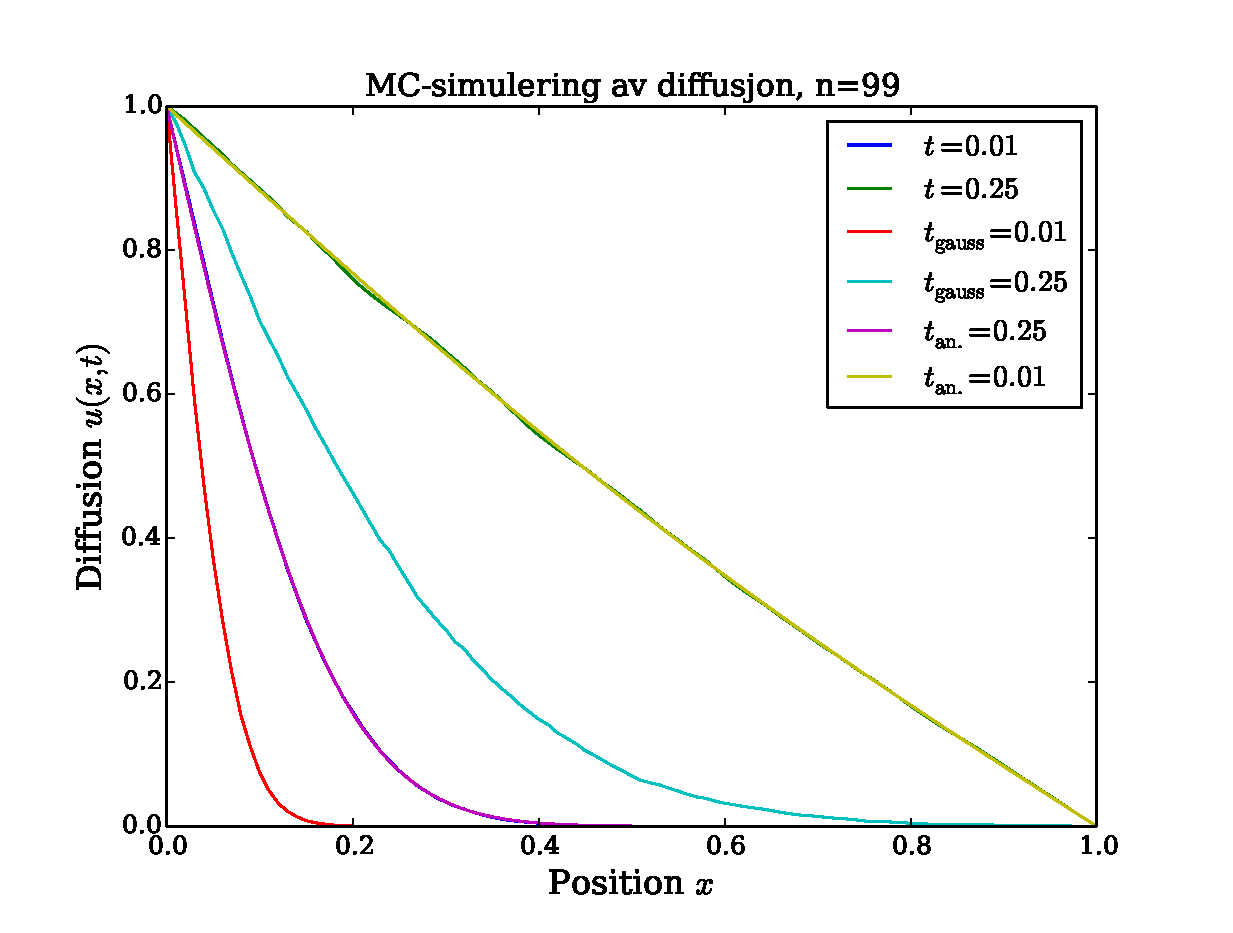
\includegraphics[scale = 0.5]{MC_walk.eps}}
\caption{}
\label{fig:analMC}
\end{figure}

% Sammenlikne MC og de andre metodene

\subsection*{Konklusjon}

\subsubsection*{Kommentarer til prosjektet}
\begin{thebibliography}{9}
%\cite{farnell}
\bibitem{farnell}
L.~Farnell,~W.G.~Gibson,
``Monte Carlo simulation of diffusion in a spatially nonhomogeneous medium: A biased random walk on an asymmetrical lattice,''
Journ.\ of Comp.\ Phys.,\ {\bf208}, (2005), 253-265, ISSN 0021-9991, \url{http://www.sciencedirect.com/science/article/pii/S0021999105001087}

%\cite{mhj}
\bibitem{mhj}
M.~H.~Jensen,
``Random walks, Brownian motion and the Metropolis algorithm,''
\url{http://compphysics.github.io/ComputationalPhysics1/doc/pub/rw/html/rw.html}, 

%\cite{mhj}
\bibitem{mhjpde}
M.~H.~Jensen,
``Partial differential equations,''
\url{http://compphysics.github.io/ComputationalPhysics1/doc/pub/pde/html/pde.html}, 


\end{thebibliography}  

\end{document}